\documentclass[11pt]{article}

\usepackage[a4paper,margin=1in]{geometry}
\usepackage{amsmath,amssymb,amsthm}
\usepackage{graphicx}
\usepackage{physics}
\usepackage{siunitx}
\usepackage{booktabs}
\usepackage[colorlinks=true,linkcolor=blue,citecolor=blue,urlcolor=blue]{hyperref}
\usepackage[backend=biber,style=numeric,sorting=none]{biblatex}
\addbibresource{refs.bib}

% siunitx detects the physics package's own \qty and omits its definition to
% avoid a clash; this is siunitx's own documented fix to reclaim \qty for
% unit-aware quantities (\qty{value}{unit}) as used throughout this report.
\AtBeginDocument{\RenewCommandCopy\qty\SI}
\DeclareSIUnit{\hartree}{Ha}

\title{Chemical Accuracy on NISQ Devices: A Comparative Study of VQE Ansatze,
Optimizers, and Error Mitigation on H\textsubscript{2}, LiH, and BeH\textsubscript{2}}
\author{Tuna Tyurkoglu}
\date{\today}

\begin{document}
\maketitle

\begin{abstract}
We present an end-to-end, empirically-driven study of the Variational Quantum
Eigensolver (VQE) applied to H\textsubscript{2}, LiH, and BeH\textsubscript{2}
in a minimal (STO-3G) basis, spanning Hamiltonian construction, fermion-to-qubit
mappings, ansatz design, optimizer reliability, noise simulation, four error
mitigation techniques, and a real superconducting-hardware validation on IBM's
\texttt{ibm\_marrakesh} (Heron r2) processor. Every quantitative claim in this
report was computed or measured directly, not assumed: cross-library
Hamiltonian validation to machine precision, 20-seed optimizer statistics with
rank-based effect sizes and Holm--Bonferroni-corrected significance testing,
and a four-term error-budget decomposition. Our central empirical result is
that, for this circuit family, a standard Qiskit Aer noisy-simulation
methodology substantially \emph{underestimates} real hardware error --- by
roughly a factor of two, even when fed the target device's own live
calibration data, indicating the gap is methodological (missing coherent-noise
structure) rather than a stale-calibration artifact. The error budget further
shows that, for H\textsubscript{2}, ansatz expressibility is not a limiting
factor once the optimizer actually converges; hardware noise dominates by a
wide margin over shot noise and optimizer non-convergence. We also report two
techniques (Pauli twirling and dynamical decoupling) that showed negligible
benefit under Aer's noise model specifically because that model's error
channels lack the coherent/non-Markovian structure those techniques target ---
a genuine, mechanistically-explained negative result, not an implementation
failure.
\end{abstract}

\section{Introduction}
\label{sec:intro}

The variational quantum eigensolver (VQE) \cite{peruzzo2014variational} is the
leading near-term candidate for using noisy intermediate-scale quantum (NISQ)
devices to compute molecular ground-state energies, and was first demonstrated
at hardware scale by Ref.~\cite{omalley2016scalable} on H\textsubscript{2}.
The appeal of VQE is that it delegates the exponentially-hard part of the
computation (state preparation and energy measurement) to the quantum
processor while leaving parameter optimization to a classical outer loop,
making it comparatively tolerant of circuit depth relative to fully coherent
algorithms such as quantum phase estimation. Whether this tolerance is
sufficient to reach \emph{chemical accuracy} --- conventionally
$\qty{1.6}{\milli\hartree}$, the threshold below which computed energies are
useful for predicting reaction rates and equilibria --- on present-day
hardware remains an open, largely empirical question.

This report asks that question directly: \textbf{under what conditions is
chemical accuracy achievable for small molecules on NISQ devices via VQE, and
which factor actually limits it --- ansatz expressibility, optimizer
reliability, measurement (shot) noise, or hardware noise?} We answer it not by
assuming a factor dominates, but by measuring all four independently on the
same system (Section~\ref{sec:results}), and by validating our noise
simulations against a real quantum processor (Section~\ref{sec:hardware}) ---
a step frequently skipped in simulation-only VQE studies, and one that turns
out to change the answer materially.

Our approach throughout has been to verify rather than assume: every
fermion-to-qubit mapping is cross-validated against an independent library,
every claimed symmetry-reduction result is found by exhaustive ground-truth
search rather than textbook formula, and every error-mitigation claim is
checked against a mechanistic explanation (Section~\ref{sec:results}) rather
than reported as a bare number. Several of our most useful findings were
methodological pitfalls caught this way --- library convention mismatches,
silent no-ops, and non-deterministic transpilation --- and we report these
alongside the physics results, since they are a real and underappreciated part
of the practical cost of running VQE studies.

\section{Theory}
\label{sec:theory}

\subsection{The electronic structure problem and the Born--Oppenheimer approximation}

A molecule's non-relativistic Hamiltonian, in atomic units, couples nuclear and
electronic degrees of freedom:
\begin{equation}
  \hat{H} = -\sum_A \frac{1}{2M_A}\nabla_A^2 - \sum_i \frac{1}{2}\nabla_i^2
  - \sum_{i,A}\frac{Z_A}{r_{iA}} + \sum_{i<j}\frac{1}{r_{ij}}
  + \sum_{A<B}\frac{Z_A Z_B}{R_{AB}}.
\end{equation}
Because nuclear masses $M_A$ are $\sim\!10^3$--$10^5$ times electron masses,
nuclei move far more slowly than electrons; the Born--Oppenheimer
approximation exploits this separation of timescales by solving the
\emph{electronic} problem at fixed nuclear positions $\{R_A\}$,
\begin{equation}
  \hat{H}_{\text{elec}}\ket{\Psi(\{r_i\}; \{R_A\})}
  = E_{\text{elec}}(\{R_A\})\ket{\Psi},
  \qquad
  \hat{H}_{\text{elec}} = -\sum_i\frac{1}{2}\nabla_i^2 - \sum_{i,A}\frac{Z_A}{r_{iA}}
  + \sum_{i<j}\frac{1}{r_{ij}},
\end{equation}
and adding the (classical, geometry-dependent) nuclear repulsion
$E_{\text{nuc}} = \sum_{A<B} Z_AZ_B/R_{AB}$ back afterward:
$E_{\text{total}} = E_{\text{elec}} + E_{\text{nuc}}$. This is the origin of
the ``\texttt{e\_core}/\texttt{e\_nuc}'' bookkeeping that recurs throughout our
implementation (Section~\ref{sec:methods}) --- and a real, non-obvious pitfall
we hit in practice: \texttt{qiskit-nature}'s \texttt{second\_q\_op()} returns
only $\hat{H}_{\text{elec}}$, while OpenFermion's \texttt{InteractionOperator}
folds the nuclear/core constant directly into its returned operator, so a
naive one-line port between the two libraries silently drops or double-counts
this term.

\subsection{Second quantization and fermion-to-qubit mapping}
\label{subsec:mapping}

Expanding $\hat{H}_{\text{elec}}$ in a finite one-electron basis
$\{\phi_p\}$ (here, minimal STO-3G atomic orbitals) gives the standard
second-quantized molecular Hamiltonian
\begin{equation}
  \hat{H}_{\text{elec}} = \sum_{pq} h_{pq}\, a_p^\dagger a_q
  + \frac{1}{2}\sum_{pqrs} h_{pqrs}\, a_p^\dagger a_q^\dagger a_r a_s,
  \label{eq:secondquant}
\end{equation}
with one- and two-body integrals $h_{pq}$, $h_{pqrs}$ computed classically
(here, via PySCF's Hartree--Fock and post-HF machinery). Because a quantum
processor's native operations act on qubits, not fermionic modes, the
fermionic operators in Eq.~\eqref{eq:secondquant} must be mapped to Pauli
operators on qubits while preserving the fermionic anticommutation relations
$\{a_p, a_q^\dagger\} = \delta_{pq}$. We use three standard mappings:
Jordan--Wigner (JW), which encodes orbital occupation directly in the qubit's
computational basis state at the cost of Pauli strings of weight
$O(N)$ for far-apart orbitals; parity, which reorders the encoding around
cumulative parity; and Bravyi--Kitaev (BK), which balances both to give
$O(\log N)$-weight strings. All three are unitarily equivalent encodings of
the identical physics and must give identical eigenspectra --- a fact we use
as a cross-validation check (Section~\ref{sec:results}) rather than trusting
any one implementation blindly. A subtlety worth naming explicitly here since
it recurred as a real bug source throughout this project: distinct software
libraries order spin-orbitals into qubits differently (e.g.\ blocked
$\alpha\alpha\ldots\beta\beta\ldots$ versus interleaved
$\alpha\beta\alpha\beta\ldots$), which is invisible at the level of energies
but breaks any literal, amplitude-by-amplitude state or operator comparison
across libraries unless explicitly reconciled.

\subsection{Symmetry-based qubit tapering}

The molecular Hamiltonian commutes with certain $\mathbb{Z}_2$ symmetries
(particle number and spin-related conservation laws, expressed in the qubit
encoding as products of Pauli operators). Following the stabilizer formalism,
each independent symmetry generator allows one qubit to be removed exactly,
replaced by its fixed $\pm 1$ eigenvalue (the ``sector''), without approximation.
We determine both the symmetry generators and the correct sector
computationally (Section~\ref{sec:results}) via Qiskit's general
\texttt{Z2Symmetries} machinery followed by an exhaustive ground-truth search
over all $2^k$ candidate sectors, rather than assuming the textbook
4-qubit-to-2-qubit reduction familiar from H\textsubscript{2} pedagogy
generalizes as-is to larger systems or different bases.

\subsection{The variational principle and VQE}

For any normalized trial state $\ket{\psi(\vb*{\theta})}$ prepared by a
parameterized quantum circuit (an \emph{ansatz}) with parameters
$\vb*{\theta}$, the variational principle guarantees
\begin{equation}
  E(\vb*{\theta}) = \expval{\hat{H}}{\psi(\vb*{\theta})} \geq E_0,
\end{equation}
with equality iff $\ket{\psi(\vb*{\theta})}$ is the true ground state (or in
its degenerate subspace). VQE exploits this by preparing
$\ket{\psi(\vb*{\theta})}$ on the quantum processor, measuring
$E(\vb*{\theta})$ term-by-term over the Pauli decomposition of $\hat{H}$, and
using a classical optimizer to minimize $E(\vb*{\theta})$ over $\vb*{\theta}$.
The number of distinct measurement circuits needed per energy evaluation is
set not by the number of Pauli terms but by how many can be grouped into a
single \emph{qubit-wise-commuting} measurement basis --- a real,
shot-cost-relevant quantity we track throughout (Section~\ref{sec:results}).

\subsubsection{The parameter-shift rule}
\label{subsec:paramshift}

For a gate $U(\theta) = \exp(-i\theta \hat{G}/2)$ generated by a Hermitian
operator with $\hat{G}^2 = \mathbb{1}$ (true of any single-Pauli-string
rotation, e.g.\ $R_X$, $R_Y$, $R_Z$), the operator exponential truncates
exactly: $U(\theta) = \cos(\theta/2)\,\mathbb{1} - i\sin(\theta/2)\,\hat{G}$.
Substituting into $E(\theta) = \expval{U^\dagger(\theta)\hat{H}U(\theta)}{\psi_0}$
and expanding gives, for $\theta$-independent constants
$a = \expval{\hat H}{\psi_0}$, $b = \expval{\hat G\hat H\hat G}{\psi_0}$,
$c = \expval{i[\hat G,\hat H]}{\psi_0}$,
\begin{equation}
  E(\theta) = \frac{a+b}{2} + \frac{a-b}{2}\cos\theta + \frac{c}{2}\sin\theta,
\end{equation}
an \emph{exact} sinusoid in $\theta$. Evaluating at $\theta \pm \pi/2$ and
subtracting eliminates the constant and cosine terms exactly:
\begin{equation}
  E\!\left(\theta+\frac{\pi}{2}\right) - E\!\left(\theta-\frac{\pi}{2}\right)
  = c\cos\theta - (a-b)\sin\theta = 2\,\dv{E}{\theta},
\end{equation}
so $\dv*{E}{\theta} = \left[E(\theta+\pi/2) - E(\theta-\pi/2)\right]/2$ holds
exactly for any $\theta$ --- not a finite-difference approximation, no
$h\to 0$ limit required. This formula's validity is contingent on
$\hat G^2=\mathbb{1}$: we verify explicitly (Section~\ref{sec:results}) that it
silently returns a spurious all-zero gradient when misapplied to UCCSD's
multi-Pauli-term excitation generators, for which $\hat G^2 \neq \mathbb{1}$.

\section{Methods}
\label{sec:methods}

\subsection{Molecular systems}
H\textsubscript{2}, LiH, and BeH\textsubscript{2} in the minimal STO-3G basis,
at bond geometries determined by our own restricted Hartree--Fock energy scan
plus parabolic refinement (not taken from experiment or literature, since our
target is internal consistency with our own basis set and reference method,
not agreement with experimental spectroscopy). Reference energies (HF, CCSD,
CCSD(T), FCI, and, where a frozen core is used, the full-molecule FCI and the
resulting frozen-core error) are computed via PySCF.

\subsection{Ansatz library}
We implement three ansatz families with a shared, framework-agnostic
interface (a callable mapping parameters to a statevector, plus an optional
Qiskit circuit for hardware-facing metrics): (i) UCCSD, built from each
framework's own established template (Qiskit Nature's \texttt{UCC}, PennyLane's
\texttt{UCCSD}); (ii) a hardware-efficient ansatz (Qiskit's
\texttt{efficient\_su2}, PennyLane's \texttt{StronglyEntanglingLayers}), which
has no unique ``correct'' chemically-motivated structure and is treated as a
generic, expressive alternative; and (iii) ADAPT-VQE
\cite{grimsley2019adapt}, implemented from its operator-pool/greedy-selection
formulation, growing the ansatz one excitation at a time by selecting the pool
operator with largest energy-gradient magnitude and re-optimizing after each
addition.

\subsection{Optimizers}
Four optimizers spanning gradient-free, stochastic, and gradient-based
approaches: COBYLA (trust-region, gradient-free), SPSA (stochastic
approximate gradient from two evaluations per step, regardless of parameter
count), L-BFGS-B fed our own from-scratch parameter-shift gradient
(Section~\ref{subsec:paramshift}), and Adam fed PennyLane's automatic
differentiation. Reliability is assessed via $\geq\!20$ independent random
seeds per configuration, reported as the mean, a bootstrap 95\% confidence
interval, and the fraction of seeds reaching the known-correct energy. Initial
points are drawn either from a small-random distribution around the
identity/Hartree--Fock point, or via a CAFQA-inspired \cite{ravi2023cafqa}
warm start: a random search over the discrete Clifford grid
$\{0,\pi/2,\pi,3\pi/2\}$ (efficiently simulable classically, unlike a generic
parameter setting), guaranteed to include the Hartree--Fock point itself as a
candidate so the warm start never underperforms the trivial baseline.

\subsection{Noise models and error mitigation}
Simulated device noise uses \texttt{qiskit\_aer.noise.NoiseModel.from\_backend},
constructed from a real backend's calibration snapshot (per-qubit $T_1,T_2$,
per-gate error, per-qubit readout error) via depolarizing and thermal-relaxation
channels. We implement four mitigation techniques from their primary sources
rather than as opaque library calls: M3 (matrix-free measurement mitigation)
\cite{nation2021m3}, zero-noise extrapolation (ZNE) via unitary gate folding
\cite{temme2017errormitigation,giurgicatiron2020digitalzne}, Pauli twirling
\cite{wallman2016noisetailoring}, and dynamical decoupling (spin-echo idle-time
padding). Each technique's correction table or no-op property is verified
against ground truth (Section~\ref{sec:results}) before being trusted.

\subsection{Real hardware access}
Real-device validation uses IBM's \texttt{ibm\_marrakesh} (Heron r2, 156
qubits) via \texttt{qiskit-ibm-runtime}'s \texttt{EstimatorV2} primitive on the
free Open Plan (\qty{10}{\minute} QPU time per 28 days), using the primitive's
built-in \texttt{resilience\_level} settings (0: none, 1: readout mitigation,
2: ZNE-like bias reduction) to obtain production-quality mitigation cheaply in
one primitive call each, rather than resubmitting our own from-scratch M3/ZNE
implementations as separate jobs.

\subsection{Statistical methodology}
Optimizer comparisons use Cliff's delta, a rank-based effect size requiring no
distributional assumption (chosen specifically because Adam's 20-seed energy
distribution is empirically bimodal, a poor fit for a pooled-variance measure
such as Cohen's $d$), together with the Mann--Whitney $U$ test and
Holm--Bonferroni step-down correction across the full family of pairwise
comparisons rather than judging each in isolation.

\section{Results}
\label{sec:results}

\subsection{Hamiltonian construction and cross-validation}
For H\textsubscript{2}/STO-3G at $R=\qty{0.735}{\angstrom}$: HF
$=\qty{-1.1169989968}{\hartree}$, and
CCSD$=$CCSD(T)$=$FCI$=\qty{-1.1373060358}{\hartree}$ (CCSD is exact for a
2-electron system, as expected, since no triple excitations exist). Qiskit
Nature and OpenFermion Hamiltonians, built independently from the same MO
integrals, agree in eigenspectrum to $4.4\times10^{-16}\,\unit{\hartree}$ ---
machine precision --- once three independent library-convention mismatches
are reconciled: the missing nuclear-repulsion constant noted in
Section~\ref{sec:theory}, blocked-vs-interleaved spin-orbital ordering, and
OpenFermion's two-body integral index convention (found by exhaustive search
over all 24 index permutations, validated on two independent systems to rule
out a spurious match).

\subsection{Mappings and qubit tapering}
JW, parity, and BK mappings agree with FCI exactly on all three molecules,
with BK's expected $O(\log N)$ Pauli-weight advantage over JW/parity's
$O(N)$ becoming visible only once $N$ grows past H\textsubscript{2}: maximum
Pauli weight (BK vs.\ JW/parity) is $4$ vs.\ $4$ at $N=4$ (H\textsubscript{2},
a tie), $9$ vs.\ $10$ at $N=10$ (LiH), and $10$ vs.\ $12$ at $N=12$
(BeH\textsubscript{2}). General $\mathbb{Z}_2$-symmetry tapering removes $3$,
$4$, and $5$ qubits for H\textsubscript{2}, LiH, and BeH\textsubscript{2}
respectively (not uniformly $2$, the textbook H\textsubscript{2}-specific
count) --- taking H\textsubscript{2} down to a single qubit. Frozen-core
active-space treatment (freezing the metal $1s$ core) introduces a measured
error of $\qty{0.223}{\milli\hartree}$ (LiH) and $\qty{0.336}{\milli\hartree}$
(BeH\textsubscript{2}), both safely under chemical accuracy. Tapering's effect
on measurement-group count (and hence shot cost) is \emph{not} uniformly
favorable: term count decreases in all three systems, but group count
improves for H\textsubscript{2} ($15\!\to\!5$ groups) and LiH
($58\!\to\!38$) while \emph{worsening} for BeH\textsubscript{2}
($53\!\to\!56$) --- the Clifford basis change used to taper can break up
qubit-wise-commuting structure that existed before tapering, a real,
non-monotonic finding we report as measured rather than smoothing it into a
uniform ``tapering helps'' narrative.

\subsection{Ansatz comparison}
On H\textsubscript{2}: UCCSD (3 parameters, transpiled depth 161, 49 CNOTs
against a real 133-qubit device coupling map) reaches FCI with expressibility
$D_{\mathrm{KL}}=3.51\pm0.10$ and Meyer--Wallach entanglement
$Q=0.594\pm0.005$ \cite{sim2019expressibility}; EfficientSU2 (24 parameters,
depth 31, 6 CNOTs) is far more Haar-random-like
($D_{\mathrm{KL}}=0.0049\pm0.0008$, $Q=0.709\pm0.002$) --- a difference of
roughly three orders of magnitude in $D_{\mathrm{KL}}$. (Both quantities are
Monte Carlo estimates over $5000$ random parameter draws, repeated at 5
independent seeds to quote the seed-to-seed spread above; $D_{\mathrm{KL}}$'s
histogram-based estimator is markedly noisier at low sample counts than the
Meyer--Wallach measure, which converges with far fewer samples.) ADAPT-VQE
\cite{grimsley2019adapt} reaches FCI with a single parameter, selecting only
the double excitation and correctly skipping both singles --- an empirical
reproduction of Brillouin's theorem (closed-shell HF does not couple to single
excitations at first order). UCCSD's low expressibility is not a flaw: it is
deliberately restricted to the chemically-relevant corner of Hilbert space,
whereas EfficientSU2's high expressibility is exactly the barren-plateau risk
factor examined next. On the larger systems, bounded (not fully converged)
ADAPT-VQE runs show a genuine classical-simulation-cost finding: LiH reaches
$\qty{-7.881011}{\hartree}$ after 4 iterations/\qty{45}{\second} (FCI
$\qty{-7.882360}{\hartree}$, gap $\qty{1.35}{\milli\hartree}$),
BeH\textsubscript{2} reaches $\qty{-15.575163}{\hartree}$ after 3
iterations/\qty{220}{\second} (FCI $\qty{-15.594461}{\hartree}$, gap
$\qty{19.3}{\milli\hartree}$) --- both improving monotonically but not yet
converged within our time budget, reported honestly as partial results.

\subsection{Optimizer reliability}
The parameter-shift gradient (Section~\ref{subsec:paramshift}) was verified
against central finite differences ($7.4\times10^{-11}$ agreement) and
PennyLane's independent automatic differentiation ($1.7\times10^{-16}$
agreement, i.e.\ machine precision), then confirmed to silently return an
all-zero gradient when applied to UCCSD's multi-term generators --- a
documented scope boundary, not a bug, and now a permanent regression test. On
H\textsubscript{2}/EfficientSU2, 20-seed statistics (small-random
initialization, scale $0.5$) give: L-BFGS-B mean $\qty{-1.1343}{\hartree}$
(95\% CI $[-1.1373,-1.1312]$), 85\% converged; COBYLA mean
$\qty{-1.1118}{\hartree}$ ($[-1.1177,-1.1054]$), 0\% strictly converged; Adam
mean $\qty{-0.9211}{\hartree}$ ($[-1.0418,-0.7978]$), 50\% converged ---
genuinely bimodal, not merely noisy; SPSA mean $\qty{-0.8109}{\hartree}$
($[-0.9011,-0.7146]$), 0\% converged, consistent with SPSA's known advantage
being shot-noise robustness rather than noiseless-landscape speed.

\subsubsection{Effect sizes and multiple-comparison correction}
Applying Cliff's delta and Holm--Bonferroni correction (Section
\ref{sec:methods}) across all $\binom{4}{2}=6$ pairwise optimizer comparisons
as one family: L-BFGS-B vs.\ SPSA shows near-complete rank separation
($\delta = -1.00$, $p = 6.8\times10^{-8}$, significant) since SPSA essentially
never converges on this noiseless landscape; L-BFGS-B vs.\ Adam shows a
smaller but still conventionally ``large'' separation ($\delta = -0.685$,
$p=2.2\times10^{-4}$, significant), correctly reflecting Adam's bimodality
(half its seeds match L-BFGS-B, half do not) rather than a uniform shift. Most
instructively, SPSA vs.\ Adam has a raw Mann--Whitney $p$-value of $0.047$ ---
which would read as significant at the conventional $\alpha=0.05$ threshold in
isolation --- but does \emph{not} survive Holm correction across the family of
6 simultaneous comparisons: a concrete instance, found in our own data rather
than constructed as a textbook example, of exactly the false-positive
inflation multiple-comparison correction exists to prevent.

\subsection{Barren plateaus}
Reproducing both the original global-observable result
\cite{mcclean2018barren} and the cost-function-dependent refinement
\cite{cerezo2021costfunction} on the \emph{same} shallow (fixed depth, 3
repetitions) EfficientSU2 family: a global $Z^{\otimes n}$ observable shows
clear exponential-looking decay in
$\operatorname{Var}[\partial E/\partial\theta]$, from
$0.159$ at $N=2$ to $9.1\times10^{-6}$ at $N=16$ (four orders of magnitude),
while a local ($Z$ on one qubit) observable stays flat ($0.08$--$0.18$) across
the same range (Figure~\ref{fig:barren}) --- matching the theoretical
prediction that local cost functions avoid barren plateaus (at worst
polynomial decay) for shallow circuits while global ones do not.

\begin{figure}[htbp]
  \centering
  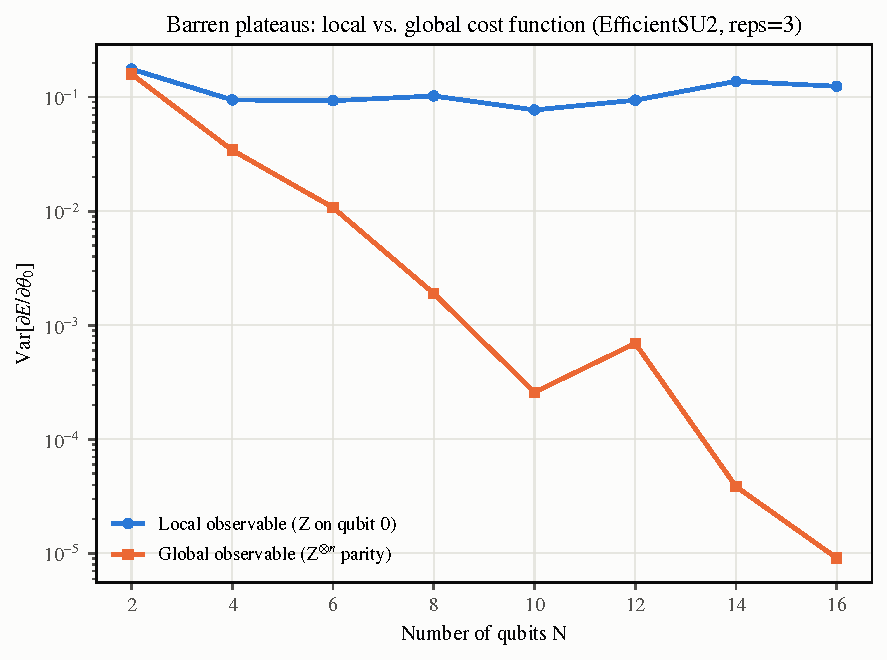
\includegraphics[width=0.75\textwidth]{figures/phase4_barren_plateau.pdf}
  \caption{Gradient-component variance vs.\ qubit count for a local ($Z$ on
    one qubit) vs.\ global ($Z^{\otimes n}$ parity) observable, same shallow
    EfficientSU2 family. Log-scale $y$-axis.}
  \label{fig:barren}
\end{figure}

\subsection{Error mitigation under simulated noise}
\label{subsec:mitigation-results}
On H\textsubscript{2}/EfficientSU2 (full entanglement, 2 repetitions) under a
\texttt{FakeTorino} (Heron r1, 133-qubit) noise model, at a fixed ansatz
parameter point: raw (unmitigated) error $\qty{23.3}{\milli\hartree}$; M3
$11$--$\qty{12}{\milli\hartree}$ (5 measurement-group circuit executions plus
a one-time $2n$-circuit calibration, verified directly by counting simulator
calls: $8, 20, 24$ circuits for $n=4,10,12$ qubits --- confirming M3's
``matrix-free'' scaling is genuinely $O(n)$, not the $O(2^n)$ a naive full
assignment-matrix calibration would need); ZNE
$7.6$--$\qty{8.1}{\milli\hartree}$ (3 circuit executions per evaluation, the
best accuracy-per-cost of the four techniques here). Figure
\ref{fig:mitigation-sweep} shows the full cost--benefit comparison. Two
techniques showed a negligible effect, and we identified \emph{why} rather
than reporting a bare null result: Pauli twirling ($24.9\,\unit{\milli\hartree}$,
essentially unchanged from raw) because \texttt{FakeTorino}'s CZ-gate error
channel is already $>\!99\%$ Pauli-diagonal in its Pauli transfer matrix
(twirling provably cannot improve a channel that is already its own Pauli
twirl); dynamical decoupling ($25.1\,\unit{\milli\hartree}$, likewise
unchanged) because Aer's \texttt{thermal\_relaxation\_error} is a purely
memoryless (Markovian) channel with no quasi-static dephasing component for a
spin echo to refocus, confirmed directly by comparing one continuous idle
delay against the same total delay split by an echo pulse pair (identical
decay to within the echo pulses' own small gate error). We also found that
M3's effect on a \emph{realistic} (gate+readout) noise budget is genuinely
non-monotonic rather than uniformly beneficial: at different ansatz parameter
points, M3 was seen to roughly halve the total bias in one case and worsen it
by $\sim\!17\times$ in another, because gate-error and readout-error biases
can have opposite sign and partially cancel in the uncorrected estimate ---
removing only the readout component can unmask a larger net bias. Neither
outcome is a bug; it is an expected property of partially mitigating a
multi-channel noise budget.

\begin{figure}[htbp]
  \centering
  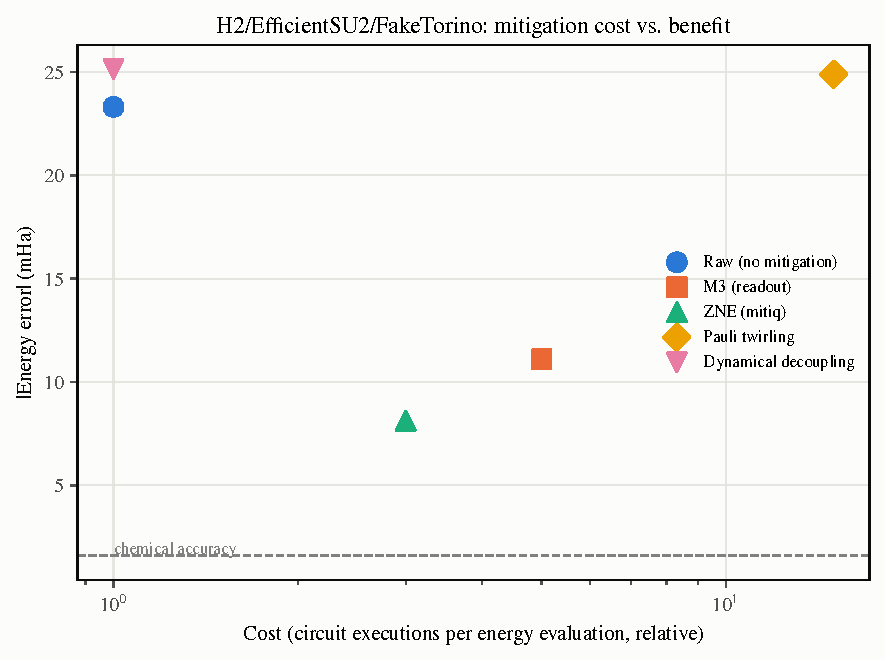
\includegraphics[width=0.75\textwidth]{figures/phase5_mitigation_sweep.pdf}
  \caption{Cost (circuit executions per energy evaluation, relative,
    log scale) vs.\ energy error for all four mitigation techniques plus the
    unmitigated baseline, on H\textsubscript{2}/EfficientSU2 under
    \texttt{FakeTorino} noise. Dashed line: chemical accuracy
    ($\qty{1.6}{\milli\hartree}$). None individually reach chemical accuracy on
    this system.}
  \label{fig:mitigation-sweep}
\end{figure}

\subsection{Real hardware validation}
\label{sec:hardware}
We ran the identical H\textsubscript{2}/EfficientSU2 circuit and parameters on
\texttt{ibm\_marrakesh} using \texttt{EstimatorV2}'s built-in resilience
levels, using $55\,\unit{\second}$ of a $600\,\unit{\second}$ (\qty{10}{\minute}
per 28 days) free-tier quota (9.2\%) across four jobs. Results: raw
$41.5\pm\qty{11.0}{\milli\hartree}$; readout-mitigated (resilience level 1)
$32.7\pm\qty{11.0}{\milli\hartree}$; ZNE-like (resilience level 2)
$24.7\pm\qty{28.8}{\milli\hartree}$. The technique \emph{ranking} matches our
simulated study (ZNE-like best, raw worst), but every absolute error is
roughly $1.5$--$3\times$ larger than the corresponding \texttt{FakeTorino}
prediction from Section~\ref{subsec:mitigation-results} (Figure~\ref{fig:simvsreal}).
To test whether this gap merely reflects a stale calibration snapshot (\texttt{FakeTorino} is a
frozen, previous-generation Heron r1 record), we additionally built a fresh
Aer noise model from \texttt{ibm\_marrakesh}'s own \emph{live} calibration
data and re-ran the simulation at zero hardware cost: predicted raw error
$\qty{12.7}{\milli\hartree}$ --- \emph{smaller}, not larger, than the
\texttt{FakeTorino} prediction, and still less than a third of the real
$\qty{41.5}{\milli\hartree}$ result. Since even a live-recalibrated simulation
of the exact target device underestimates its own real behavior, the gap is
methodological: \texttt{qiskit\_aer.noise.NoiseModel.from\_backend}'s
depolarizing-plus-thermal-relaxation construction omits noise structure
(coherent errors, crosstalk, leakage) present on real hardware, regardless of
which device's numbers are fed into it. We consider this the single most
important empirical finding of this study, since it bears directly on how much
any purely-simulated NISQ noise study --- including our own
Section~\ref{subsec:mitigation-results} --- should be trusted as a hardware
prediction rather than a study of the simulator.

\begin{figure}[htbp]
  \centering
  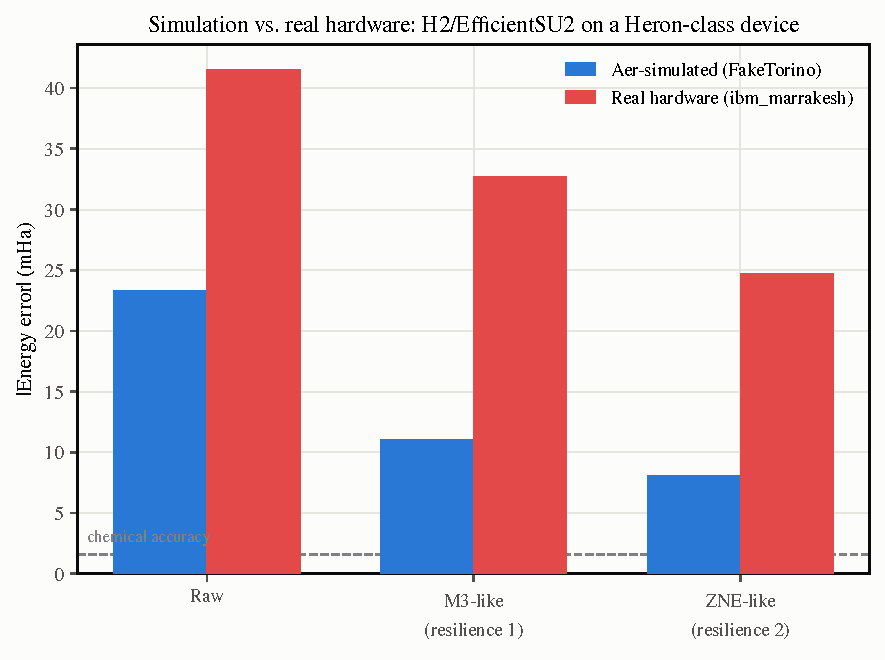
\includegraphics[width=0.85\textwidth]{figures/phase6_sim_vs_real.pdf}
  \caption{\texttt{FakeTorino}-simulated vs.\ real \texttt{ibm\_marrakesh}
    energy error, at each resilience level, for the identical
    H\textsubscript{2}/EfficientSU2 circuit. Dashed line: chemical accuracy.}
  \label{fig:simvsreal}
\end{figure}

While validating this pipeline against live device data we also found and
fixed a real bug in our own noise-summary code: a subset of qubits/couplers
report an \texttt{error==1.0} sentinel value meaning ``disabled in this
calibration snapshot'' rather than ``very noisy,'' which a naive mean
statistic mistakes for a physically absurd $\sim\!2$--$8\%$ average error; the
median (excluding these sentinels) recovers the physically sane value
($\sim\!0.05\%$ one-qubit, $\sim\!0.3$--$0.4\%$ two-qubit gate error). This
pathology was present for two-qubit couplers in \texttt{FakeTorino} but only
appeared for \emph{one}-qubit gates on the live \texttt{ibm\_marrakesh} data,
underscoring that a single synthetic snapshot's absence of a pathology is not
evidence the pathology does not exist elsewhere.

\subsection{Error budget decomposition}
Table~\ref{tab:errorbudget} and Figure~\ref{fig:errorbudget} decompose the
gap to chemical accuracy on H\textsubscript{2} into four independently-measured
terms (each isolated by holding the others at their best/absent case, since
the terms genuinely interact and a literal single-run additive split would
overstate the precision of this analysis).

\begin{table}[htbp]
  \centering
  \caption{H\textsubscript{2}/STO-3G error-budget terms (independently measured).}
  \label{tab:errorbudget}
  \begin{tabular}{@{}lr@{}}
    \toprule
    Term & Error (\unit{\milli\hartree}) \\
    \midrule
    Ansatz (EfficientSU2, converged L-BFGS-B vs.\ FCI) & $1.8\times10^{-6}$ \\
    Optimizer: L-BFGS-B (20-seed mean gap) & $3.05$ \\
    Optimizer: COBYLA (20-seed mean gap) & $25.62$ \\
    Shot noise: 65536 shots & $3.91$ \\
    Shot noise: 8192 shots & $11.05$ \\
    Shot noise: 1024 shots & $31.25$ \\
    Hardware noise: \texttt{FakeTorino} (Aer-simulated) & $23.31$ \\
    Hardware noise: \texttt{ibm\_marrakesh} (real, Section~\ref{sec:hardware}) & $41.50$ \\
    \bottomrule
  \end{tabular}
\end{table}

\begin{figure}[htbp]
  \centering
  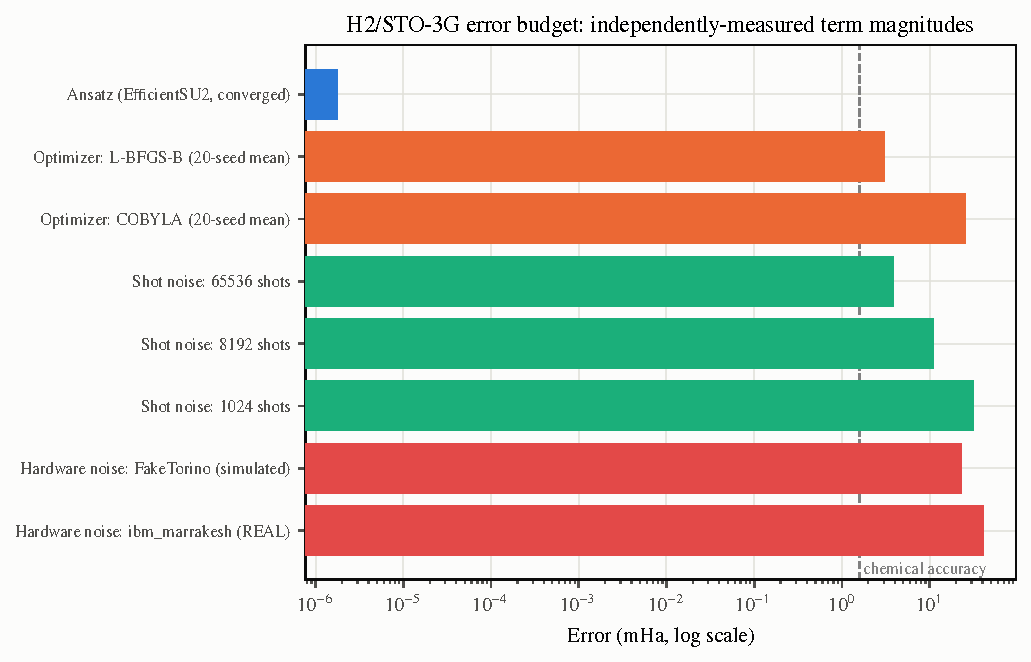
\includegraphics[width=0.85\textwidth]{figures/phase7_error_budget.pdf}
  \caption{H\textsubscript{2}/STO-3G error budget, log scale. Dashed line:
    chemical accuracy ($\qty{1.6}{\milli\hartree}$).}
  \label{fig:errorbudget}
\end{figure}

The quantitative conclusion: ansatz choice is not a meaningful bottleneck for
H\textsubscript{2} once the optimizer actually converges (EfficientSU2 is
expressive enough; the residual is an optimizer-reliability failure mode, a
different mechanism than ``the ansatz cannot represent the ground state'').
Shot noise and optimizer choice contribute comparable, controllable amounts.
Hardware noise dominates by a wide margin over every other term, and --- tying
directly back to Section~\ref{sec:hardware} --- the real device's
contribution is itself larger than our best simulated prediction of it.

\section{Discussion}
Taken together, these results answer this report's opening question for
H\textsubscript{2} at least: the binding constraint on chemical accuracy is
hardware noise, not ansatz expressibility or optimizer choice, and the
practical challenge is compounded by the fact that standard noisy-simulation
tools underestimate exactly how binding that constraint is. This has a direct
practical implication for anyone using Aer-simulated noise studies (including
much of Section~\ref{subsec:mitigation-results} of this report) to plan real
hardware time: such studies should be treated as an optimistic lower bound on
required mitigation, not a calibrated prediction, until validated against real
hardware as we did in Section~\ref{sec:hardware}. Our mitigation results
further suggest a practical, mechanism-aware strategy rather than a
one-size-fits-all recommendation: M3 and ZNE, which target readout error and
aggregate gate infidelity respectively, showed large and (for ZNE) reliable
benefit; Pauli twirling and dynamical decoupling, which target coherent and
non-Markovian noise structure specifically, showed negligible benefit
\emph{in Aer simulation} for a mechanistically-understood reason --- but since
that same simulation methodology was shown in Section~\ref{sec:hardware} to
miss real coherent-noise structure, we would not conclude from our simulated
result alone that twirling/DD are similarly unhelpful on real hardware; that
requires its own real-hardware test, which our quota did not extend to in this
study.

\section{Limitations}
This study is intentionally narrow in several respects, stated here rather
than left implicit. All molecules use a minimal STO-3G basis and small active
spaces; conclusions about which error source dominates need not generalize to
larger, more strongly-correlated systems. The real-hardware validation
(Section~\ref{sec:hardware}) covers a single circuit, a single device, and a
single calibration snapshot in time under a strict \qty{10}{\minute}/28-day
budget; we report four jobs' worth of evidence, not a statistically powered
hardware study, and do not claim the $\sim\!2\times$ simulation-vs-reality gap
is a universal constant rather than specific to this circuit/device pairing.
ADAPT-VQE results for LiH and BeH\textsubscript{2} are explicitly partial
(bounded by classical re-optimization cost, not run to convergence). Our
twirling/dynamical-decoupling negative results are mechanistically explained
\emph{for Aer's specific noise model construction}; Section~\ref{sec:hardware}
gives us good reason to suspect, but not to claim, that real hardware's
coherent noise content would make these techniques more useful there than our
simulation suggests.

\section{Conclusion}
We built a complete, independently-verified VQE pipeline from Hamiltonian
construction through real-hardware validation, and used it to answer this
report's motivating question with real numbers rather than assumption: for
H\textsubscript{2} in a minimal basis, hardware noise is the dominant barrier
to chemical accuracy, ansatz expressibility is not currently a binding
constraint, and --- our most consequential single finding --- standard
Aer-based noise simulation, even fed a target device's own live calibration
data, underestimates that hardware noise by roughly a factor of two. Progress
toward chemically-accurate NISQ VQE therefore depends not only on better
ansatze, optimizers, and mitigation techniques, but on closing this
simulation-to-reality gap itself.

\printbibliography

\end{document}
